\chapter{Analyse}\label{ch:analyse}

Um ein konkretes Lösungskonzept zu entwickeln, musste die bestehende App zunächst analysiert werden. Im Folgenden werden die verschiedenen Aspekte dieser Phase erläutert, um anschließend in \Cref{ch:konzept} die konkreten Lösungskonzepte vorzustellen.

\section{Struktur des Couchbase-Datenbank-Frameworks}\label{sec:couchbase-framework}

Für die Persistierung von Daten bieten sich eine Vielzahl von Möglichkeiten. Während sich kleinere Datenmengen (< 1.42 MB) für nutzerbezogene Daten bereits in den \texttt{SharedPreferences}\footnote{SharedPreferences. \url{https://developer.android.com/reference/android/content/SharedPreferences}} speichern lassen, so bietet die Android-Platform mit \texttt{Room}\footnote{Room. \url{https://developer.android.com/training/data-storage/room}} eine umfängliche Bibliothek zur Erstellung von SQLite-Datenbanken. Eine Funktionalität die beiden Implementationen allerdings fehlt, ist die Synchronisierung mit einem Remote-Server. Zeitgleich sollten die Daten lokal persistiert werden, um die App auch ohne Internetzugriff vollständig bedienen zu können. Aus diesen Anforderungen ergeben sich nur eine geringe Anzahl an Frameworks, die für die Nutzung im Rahmen der OUTPUT-App zutreffend sind. Da die Nutzungskonditionen des Dienstes Realm starke Limitationen aufweisen, fiel die Entscheidung zukünftig stattdessen das Framework Couchbase verwenden zu wollen. Aus diesem Grund wurden im Verlauf des Sommersemesters 2020 Datenbank-Frameworks erstellt, welche die Bereitstellung von Daten für die App sowie die notwendige Synchronisationsfunktion beinhalten. Um die Komplexität des Couchbase-Frameworks zu Kapseln abstrahieren die Bibliotheken Zugriffe auf die Dokumente sowie Serialisierung und Deserialisierung von Daten und stellen den jeweiligen Apps damit eine Schnittstelle für den Datenzugriff zur Verfügung. Die zentrale Idee hinter der Umsetzung bildete das Repository-Pattern. Dabei stehen Operationen zum Erstellen, Lesen, Schreiben und Löschen von Daten zur Verfügung, während die zugrunde liegende Implementierung des Couchbase-Frameworks versteckt wird. Die Metastruktur des Frameworks ist in \Cref{fig:couchbase-framework} gezeigt.

\begin{figure}[H]
    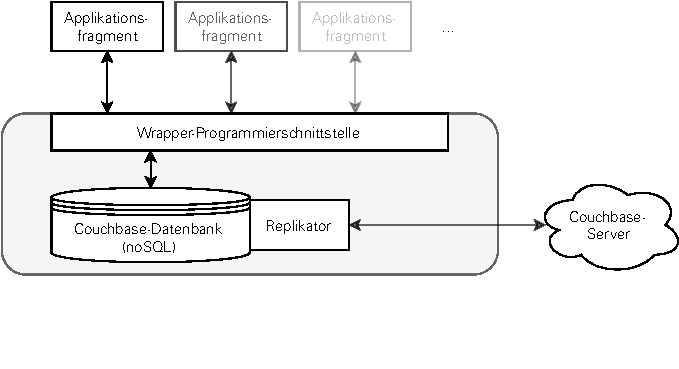
\includegraphics[width=1\linewidth]{31-couchbase-framework.pdf}
    \vspace{-25mm}
    \caption{Bereitstellung einer Bibliothek für die Abstraktion von Datenbank-Operationen mittels Couchbase.}\label{fig:couchbase-framework}
\end{figure}


Um die in Dokumenten abgelegten Daten in ein objektorientiertes Schema überführen zu können, entschieden wir uns einen sogenannten
\texttt{DocumentIdentifier} hinzuzufügen. Diese Zeichenkette wird als Teil des Serialisierungsprozess im Dokument gespeichert und dient im folgenden zur Abgrenzung einzelner Modell-Klassen. Damit lassen sich Objekte eines bestimmten Typs von der Datenbank lesen um bspw. einen Veranstaltungsplan zu erzeugen. Des Weiteren wird die Eigenschaft des (zusammengesetzten) Primärschlüssel über eine Annotation im Quellcode angegeben, wodurch Objekte eindeutig identifizierbar sind. Ähnlich des Primärschlüssels können einzelne Attribute auch mittels Annotation für die Volltextsuche markiert werden, um bestimmte Schlagwörter in Texten zu finden. Mittels generischer Programmierung konnten wir erreiche, dass sämtliche Operationen durch einmalige Definition in der Basisklasse \texttt{Repository} anschließend für alle Modelle entsprechende Methoden bereitstellt, welche die notwendigen Typen automatisch inferieren kann. Somit genügen wenige Zeilen, um neue Modelle in die bestehende Repository-Architektur hinzuzufügen. Die Struktur ist in \Cref{fig:couchbase-framework-generic} gezeigt. Außerdem ist es möglich asynchrone Programmierpraktiken einzubinden, bei welchen Funktionsaufrufe in Kotlin Coroutines ausgeführt werden können.

\begin{figure}[H]
    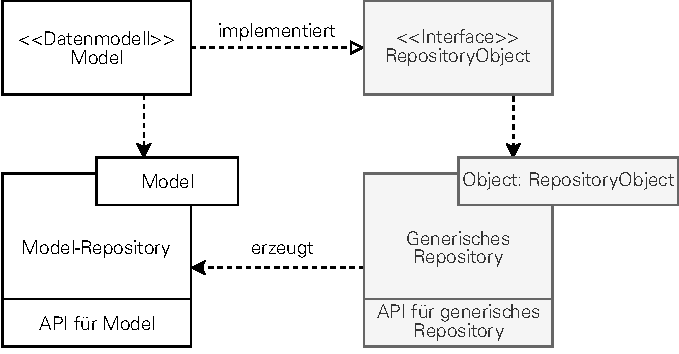
\includegraphics[width=0.85\linewidth]{32-couchbase-framework-generic.pdf}
    \caption{Generisches Konzept zur Umsetzung des Repository-Patterns für Model-Klassen.}\label{fig:couchbase-framework-generic}
\end{figure}

\section{Ermittlung einer Dialoglandkarte}\label{sec:app-architecture-mindmap}

Da die Android-App in ihrer Fassung ohne weiteres abstürzte und in sich in keinem nutzbaren Zustand befand, wurde die bestehende iOS-App analysiert. Ziel dieser Arbeit war es, eine Dialoglandkarte zu erstellen, anhand welcher die Navigationswege eines Nutzers in der App nachvollzogen werden konnte. Gleichzeitig sollte die erstellte Übersicht eine topologische Ordnung der Ansichten bieten und die genutzten UI-Elemente aufzeigen. Die in \Cref{fig:app-architecture-mindmap} abgebildete Dialoglandkarte beinhaltet bereits eine Gruppierung von Ansichten in eigenständige Teilbereiche der App, die für die nachfolgende Implementierung in separaten Komponenten nützlich war. Durch die Pfeile zwischen Ansichten konnten die Daten- und Navigationsflüsse innerhalb der App aufbereitet werden. 

\begin{figure}[H]
    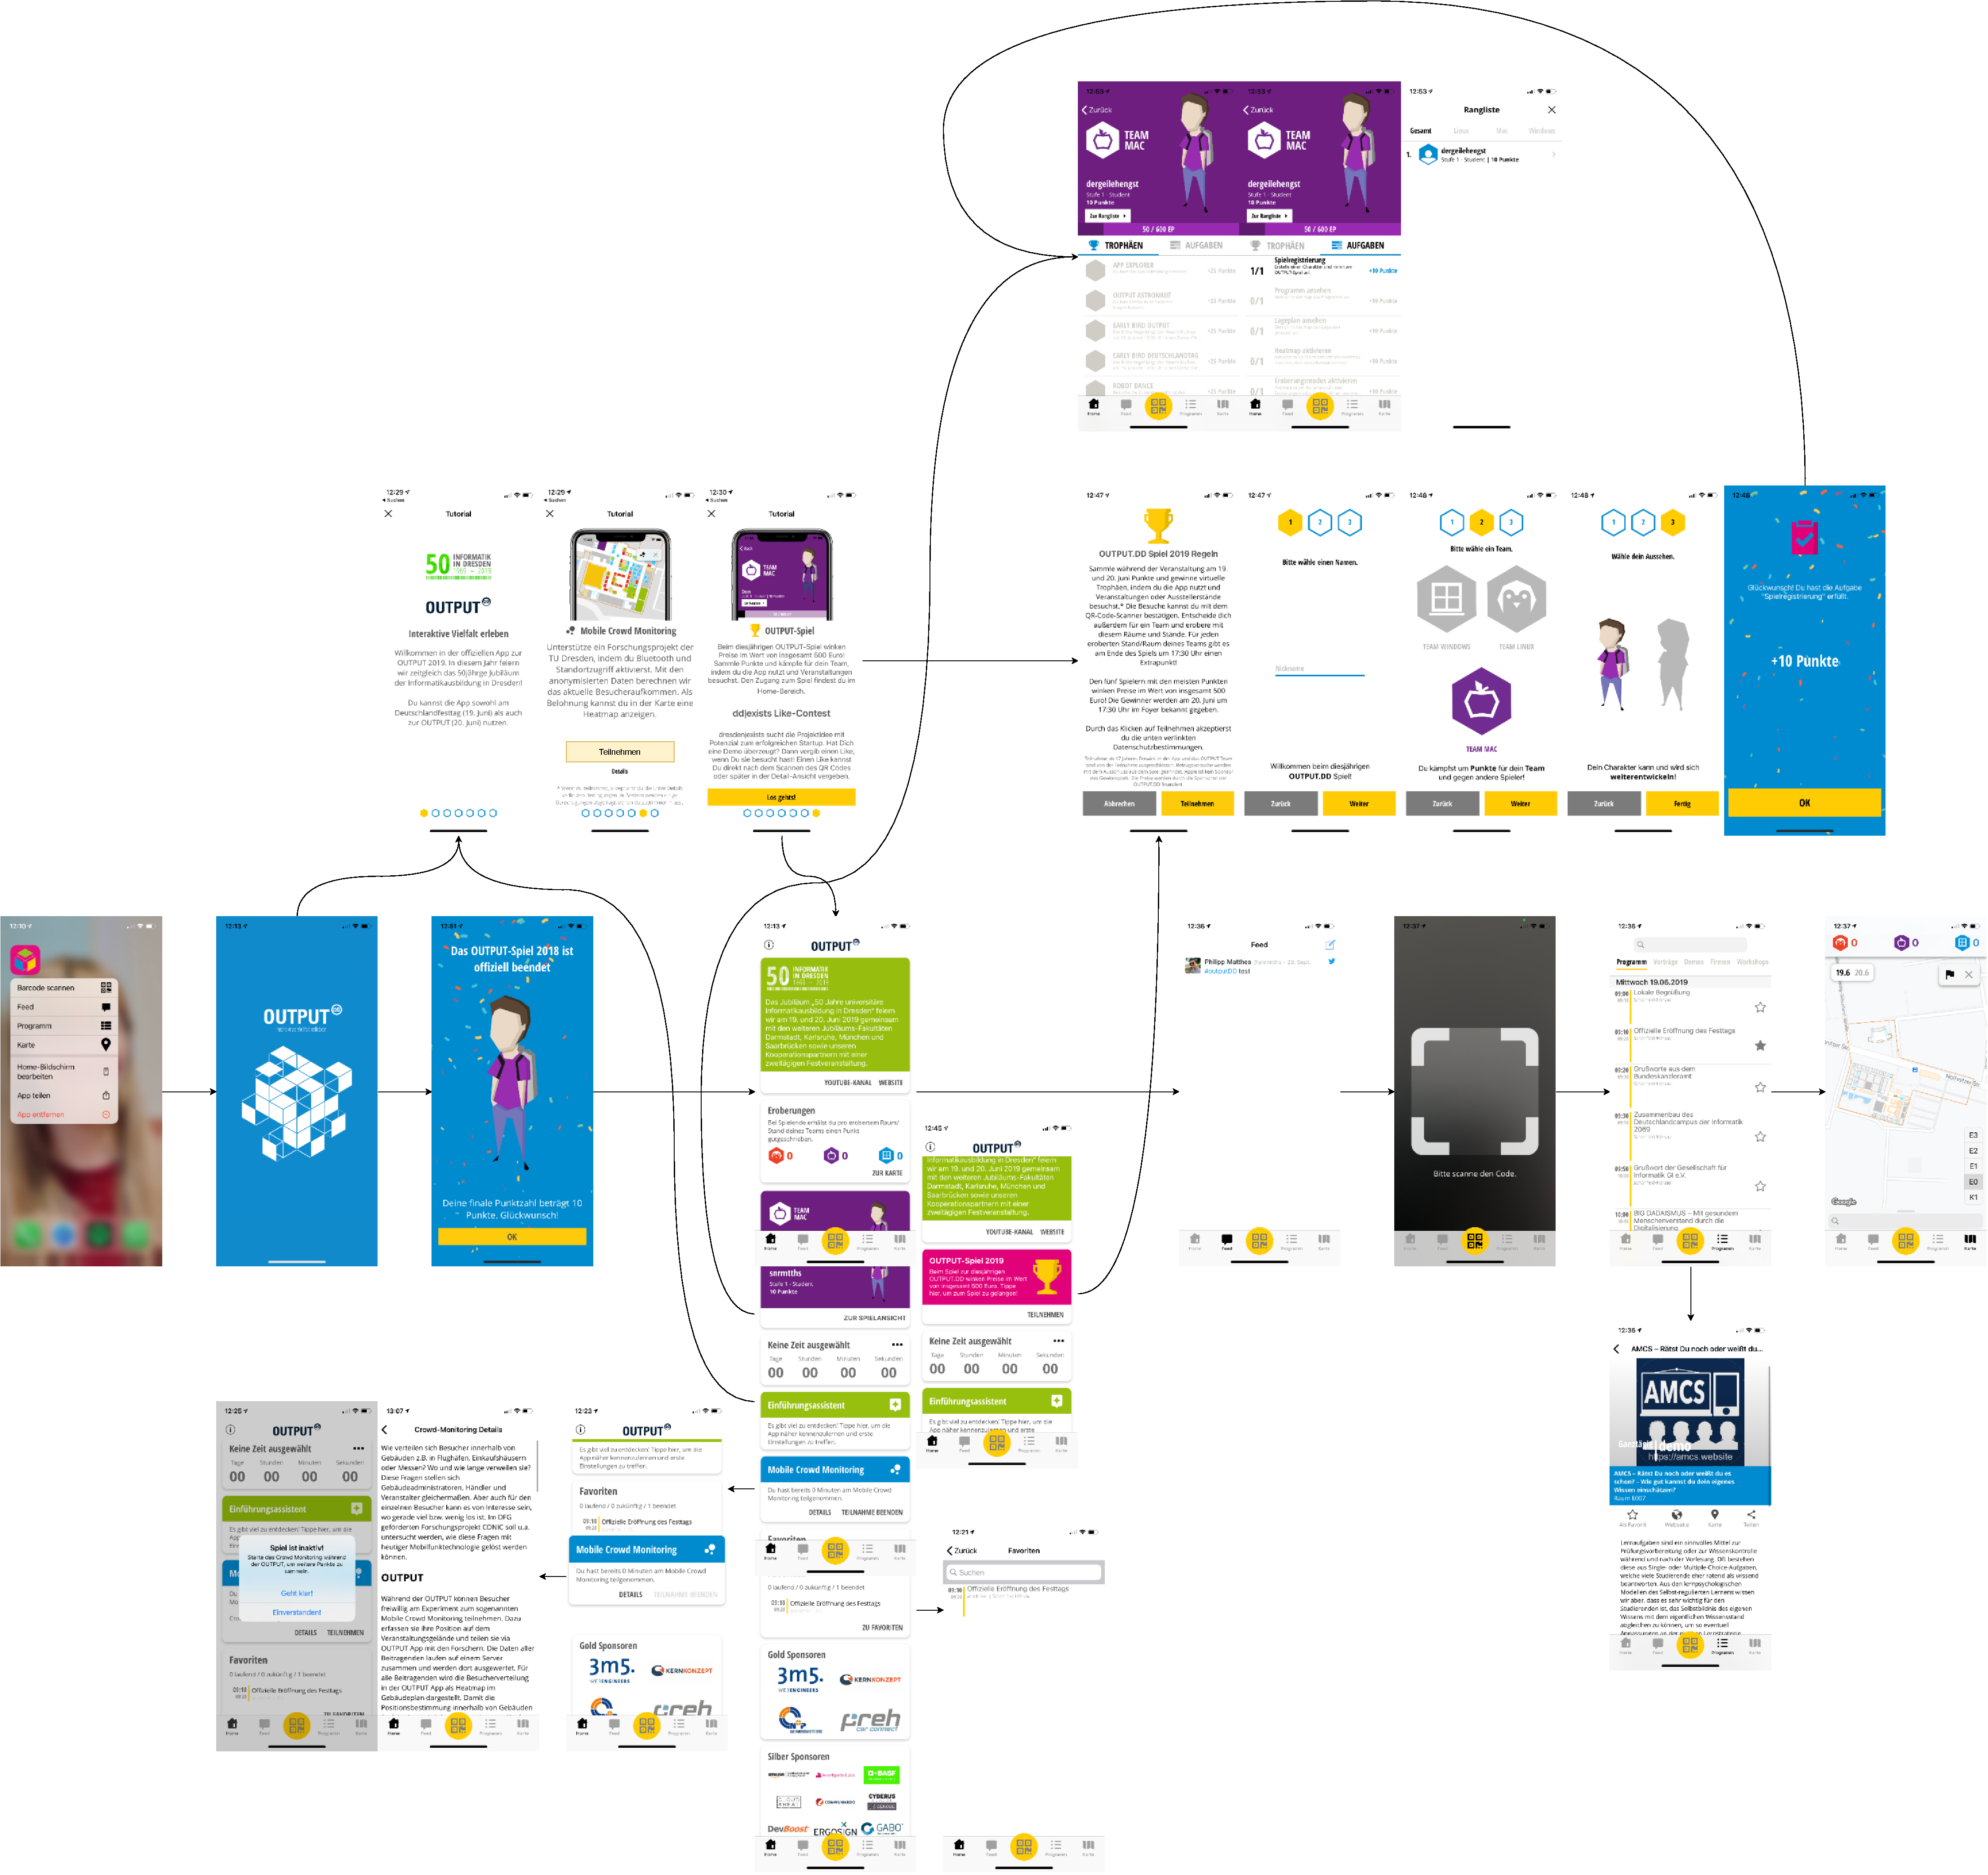
\includegraphics[width=1\linewidth]{33-app-architecture-mindmap.pdf}
    \caption{Die Dialoglandkarte zur vorangegangenen Version der iOS App.}\label{fig:app-architecture-mindmap}
\end{figure}
